\scanpage{11}
\mspage{\textcircled{5}}
% archive foliation: 10
\deleted{$\unsure{HC|H^C}$}
\diagram{\begin{tikzcd}A\arrow[r,hook,"\text{pl fid}"']&B\end{tikzcd}}
\[
x\in B\qquad H_x\in\widehat A\qquad H_x(a)=\mathrm{Hom}_B(a,x)
\]
\[
H^x\in A^\vee\qquad H^x(\cdot)=\mathrm{Hom}_B(a,x)
\]
\[
H_x(a)\times H^x(b)\xrightarrow{\alpha_x}\mathrm{Hom}_A(a,b)
\]
Soit $\unsure{\widetilde{\widetilde A}|\widetilde A}_{\deleted{\unsure{*}}}$ la catégorie des triples $(H_*,H^*,\alpha)$
\unsure{i.e.}
\[
H_*\in\widehat A,\quad H^*\in A^\vee,\quad
\alpha:H_*(a)\times H^*(b)\longrightarrow\mathrm{Hom}_A(a,b)
\]
(bifonctoriel)

les flèches
\[
(H_*,H^*,\alpha)\xrightarrow{\varphi}(H'_*,H'^*,\alpha')
\]
étant données par
\[
\left\{\begin{aligned}
\varphi_*:H_*&\longrightarrow H'_*&&\text{dans }\widehat A\\
\varphi^*:H'^*&\longrightarrow H^*&&\text{dans }A^\vee
\end{aligned}\right.
\]
tels que \deleted{\unsure{l'}} l'on ait
\margin{\diagram{\begin{tikzcd}[row sep=small,column sep=small]
a\arrow[d,"u"']\arrow[dr,"(u')"]&\\
x\arrow[r]\arrow[d,"(v)"']&x'\arrow[dl,"v'"]\\
b&
\end{tikzcd}}}
\diagram{\begin{tikzcd}[row sep=large,column sep=small]
\unsure{u\in}\ \deleted{\unsure{a}}H_*(a)\arrow[d,"\varphi_*"']&\times&H^*(b)\arrow[rr,no head,"\alpha_{a,b}"]&&\mathrm{Hom}(a,b)\arrow[d,equal]\\
H'_*(a)&\times&H'^*(b)\arrow[u,"\varphi'_*"']\arrow[rr,no head,"\alpha'_{a,b}"']&&\mathrm{Hom}(a,b)\\
&&\unsure{v'}\arrow[u,phantom,"\in" description]&&
\end{tikzcd}}
\[
\alpha_{a,b}(u,\varphi'_*(\unsure{v'|u'}))=\alpha'_{a,b}(\varphi_*(u),\unsure{v'|u'})
\]
\deleted{Soit $\unsure{A^\sim}$}
Pour un foncteur pl. fid \(A\xrightarrow{\varphi}B\), on déduit un foncteur
\[
\begin{aligned}
\varphi^{\unsure{\sharp|\natural}}:B&\longrightarrow\widetilde A\\
x&\longmapsto(\varphi^*_{\unsure{(!)}}(\unsure{a|x}),\varphi^{\circ *}(\unsure{a|x}),\alpha_x)
\end{aligned}
\]

\margin{\figure{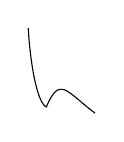
\begin{tikzpicture}\draw(0,1)..controls(.03,.5)and(.12,.05)..(.23,0)..controls(.4,.4)and(.48,.2)..(.85,-.08);\end{tikzpicture}}}
